\begin{flushleft}
	An OS consists of:
	\begin{itemize}
		\item Kernel
		\item Shell
		\item Applications
	\end{itemize}
	\begin{figure}[h!]
		\centering
		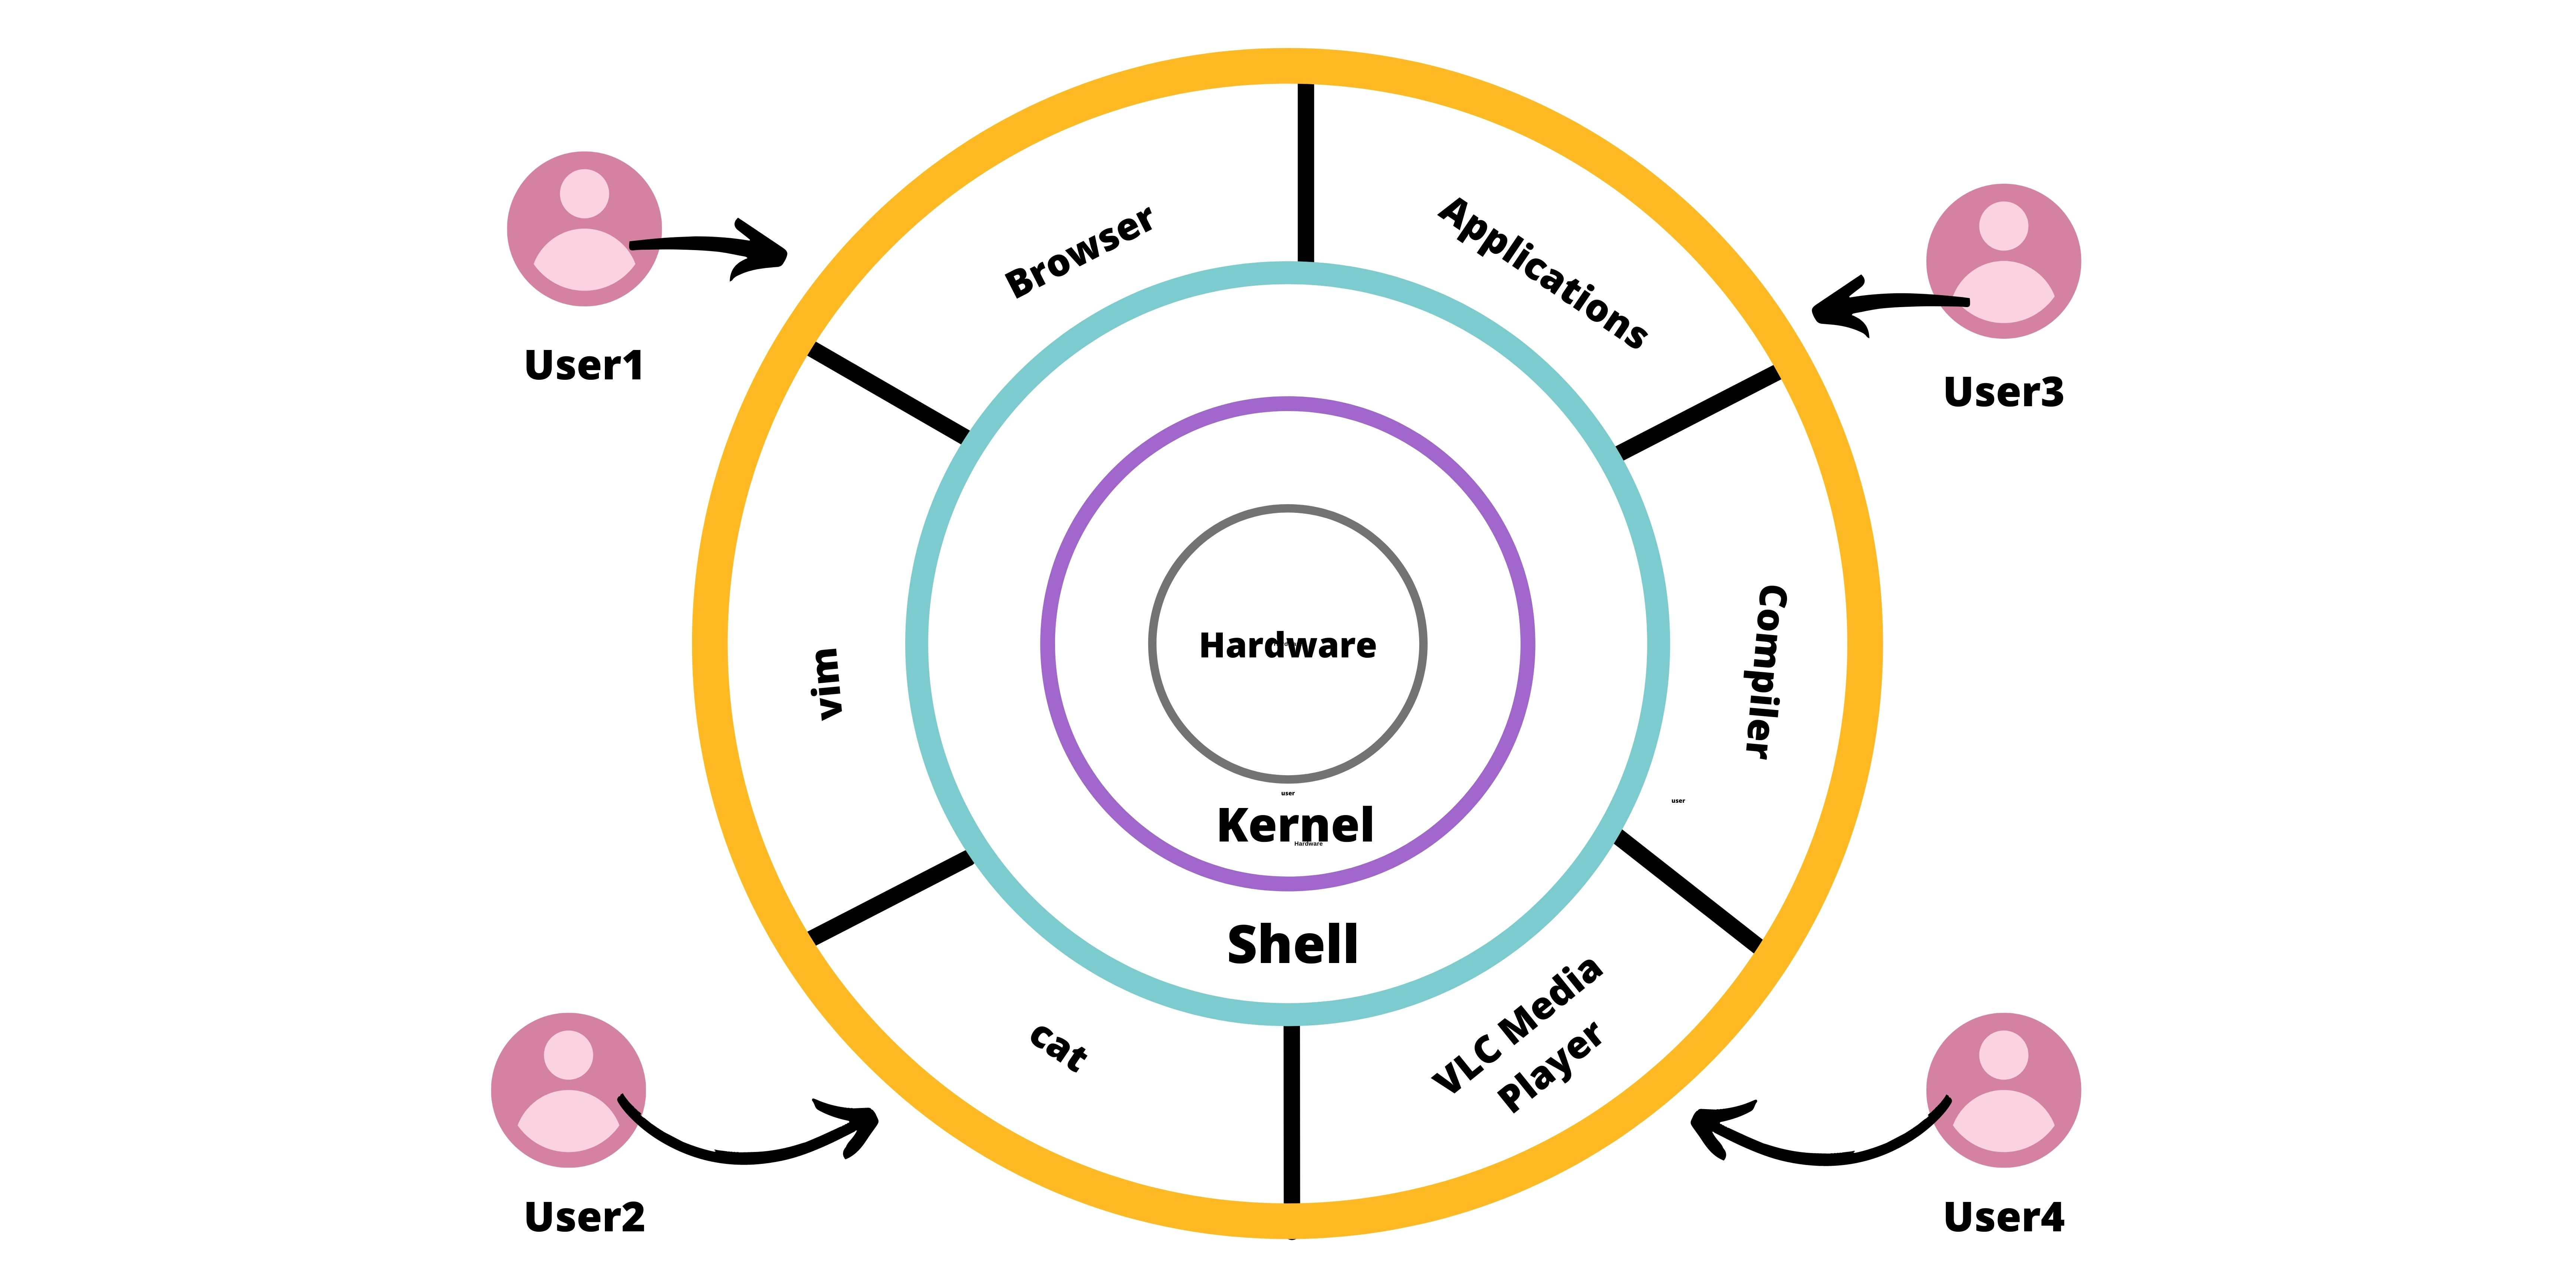
\includegraphics[scale=.08]{content/chapter1/images/os_structure.jpg}
		\caption{OS architecture}
		\label{fig:OS_Structure}
	\end{figure}
	Let's see each of these in detail.
	
	\newpage
	
	\begin{enumerate} 
		\item \textbf{Kernel} - 
		\begin{itemize}
			\item Establish communication between hardware and software.
			\begin{figure}[h!]
				\centering
				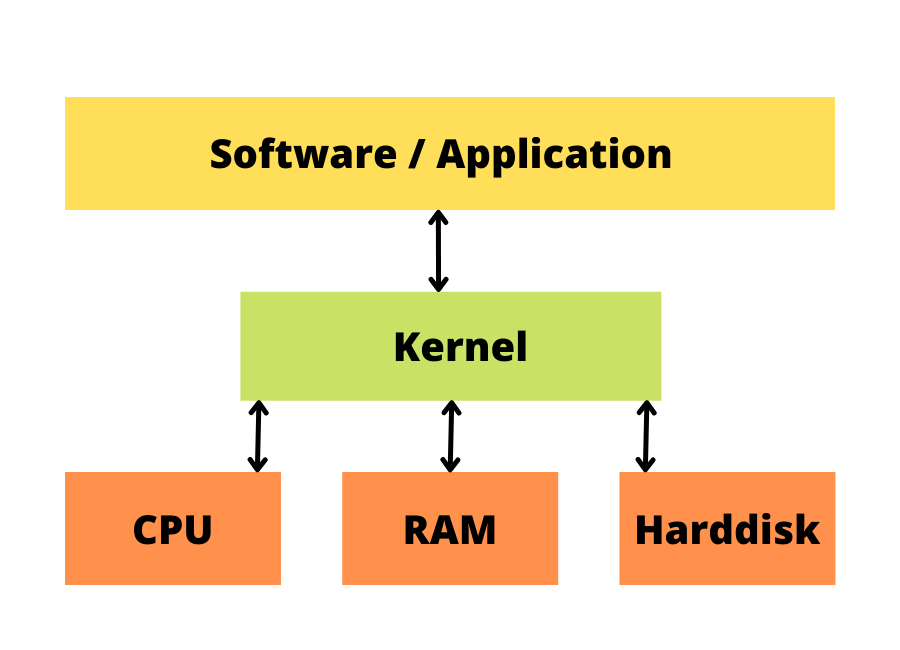
\includegraphics[scale=.4]{content/chapter1/images/kernel.png}
				\caption{Kernel}
				\label{fig:kernel}
			\end{figure}
			\item Kernel performs:
			\begin{itemize}
				\item \textbf{Process Management}: Manage CPU processes.
				\item \textbf{Device Management}: Interface between hardware and process.
				\item \textbf{Memory Management}: Manage RAM.
				\item \textbf{Handling system calls}: Provides the interface between the processes and OS.
			\end{itemize}			
		\end{itemize}
		\bigskip
		
		\item \textbf{Shell} - An interface to kernel that takes commands from user and executes them.
		\bigskip
		
		\item \textbf{Utilities/applications} - Programs that can be directly used by users.
	\end{enumerate}
\end{flushleft}

\newpage



